\chapter{MPC Implementation}

The offline intervalwise MPC presented in chapter \ref{ch:optimization} will be implemented using C++ and the ACADO Toolkit \cite{acadoHOUSKA}. The implementation conists of two main parts: the MPC algorithm that prepares the optimization problem, and the optimization solver that will use the ACADO Toolkit to solve the optimization problem.

This chapter will describe the ACADO Toolkit, how to use it and how it works; as well as the MPC algorithm. An overview of what information the modules share is shown in figure \ref{fig:sys_overview}.

\begin{figure}[h]
	\centering
    \makebox[\textwidth][c]{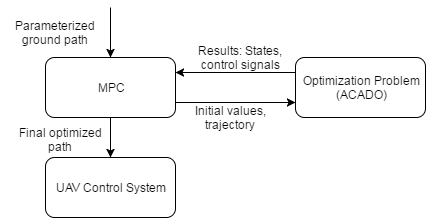
\includegraphics[width=\textwidth, keepaspectratio=true]{sys_overview.png}}
	\caption{An overview of what information the modules share.}
	\label{fig:sys_overview}
\end{figure}
	
\import{./}{acado_toolkit.tex}
\import{./}{optimization_problem.tex}
\import{./}{mpc.tex}